\subsection{Dimensionering af filter med 2.62dBs forstærkning}
\label{DimensioneringAfFilter2.62}
%
Da der arbejdes med tre RC-led er det nødvendigt dele den samlede forstærkning i dB, i tre lige store dele, som illustreret på \autoref{fig:GainOpdeling}.
%
\begin{figure}[H]
	\centering
	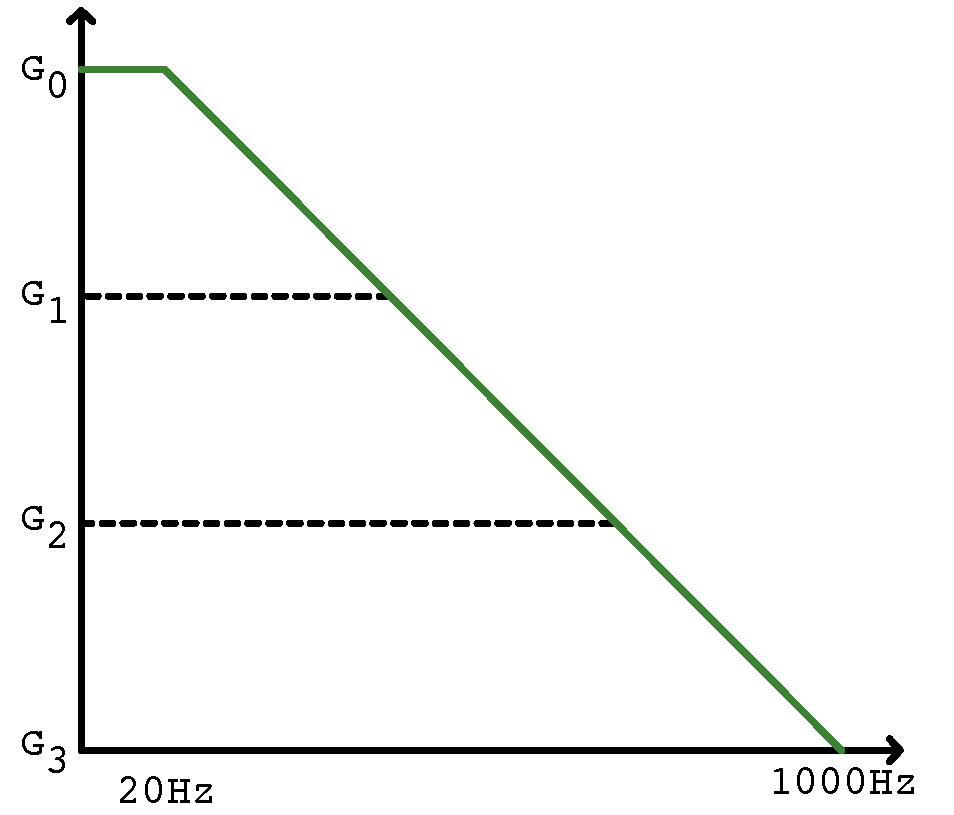
\includegraphics[resolution=300,scale=\circuitSize]{Figure/DesignAfFilter/GainOpdeling.pdf}
	\caption{Illustration af forstærkningsopdelingen, hvor x-aksen angiver frekvens og y-aksen angiver forstærkningen.}
	\label{fig:GainOpdeling}
\end{figure}
\noindent
%
Det første forstærkningstrin skal sørge for at ved 20Hz er der en forstærkning på 2.62dB og det sidste forstærkningstrin sørger for at ved 1000Hz er der en forstærkning på 0dB. De to trin derimellem sørger for at forstærkningen foregår lineært. For at få denne opdeling af forstærkning vil det først blive regnet ud i forhold til forstærkningen i dB, og derefter i forhold til råforstærkning: 
%
\begin{equation}
	G_{0(dB)} = \frac{3}{3}*2.62dB = 2.62dB
\end{equation} 
%
\begin{equation}
	G_{1(dB)} = \frac{2}{3}*2.62dB = 1.7467dB
\end{equation}
%
\begin{equation}
	G_{2(dB)} = \frac{1}{3}*2.62dB = 0.8733dB
\end{equation}
%
\begin{equation}
	G_{3(dB)} = \frac{0}{3}*2.62dB = 0dB
\end{equation}
%
Baseret på \autoref{equ:Gain} omregnes forstærkningerne i dB til den tilsvarende råforstærkning.
%
\begin{equation}
	G_0 = 10^\frac{2.62dB}{20} = 1.3521
\end{equation}
%
\begin{equation}
	G_1 = 10^\frac{1.7467dB}{20} = 1.2227
\end{equation}
%
\begin{equation}
	G_2 = 10^\frac{0.8733dB}{20} = 1.1058
\end{equation}
%
\begin{equation}
	G_3 = 10^\frac{0}{20} = 1
\end{equation}
%
For at beregne hvor store modstandende og kondensatorerne skal være i de tre tilbagekoblede RC-led, er det nødvendigt at tage et led ad gangen. 
%
\begin{figure}[H]
	\centering
	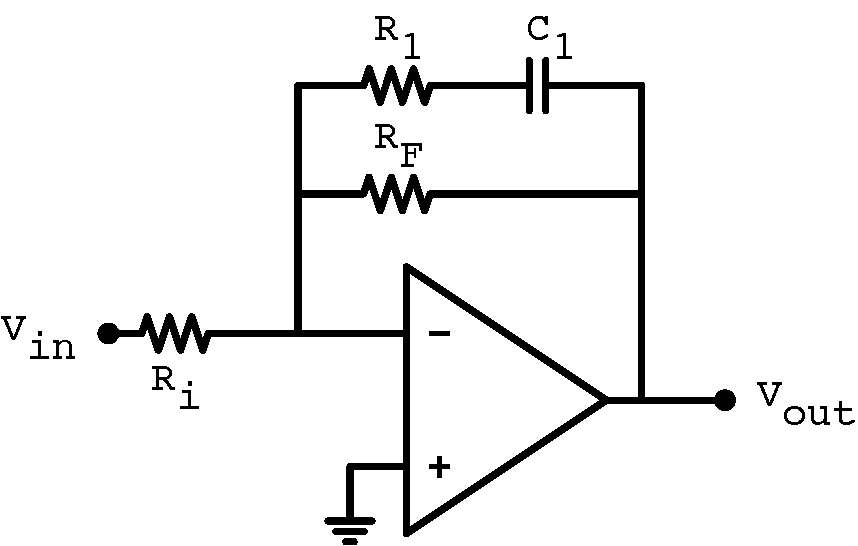
\includegraphics[resolution=300,scale=\circuitSize]{Figure/DesignAfFilter/FilterWith1.pdf}
	\caption{Kredsløbsdiagram for et lavpasfilter med et RC-led.}
	\label{fig:ELdiagramForFilter}
\end{figure}
\noindent
%
Modstanden $R_i$ vælges til 10k$\Omega$, og gør sig gældende for de efterfølgende beregninger af de tre RC-led. Den første overføringsfunktion relaterer sig til at beregne $G_0$ baseret på forholdet mellem $R_i$ og $R_F$:
%
\begin{equation}
	G_0 = -\frac{R_F}{R_i} \Rightarrow R_F = G_0*R_i
	\label{equ:Tilbagekoblingsmodstand}
\end{equation}
%
\begin{equation}
	R_F =  1.3521*10k\Omega = 13.521k\Omega
\end{equation}
%
Med udgangspunkt i et RC-led, som illustreret på \autoref{fig:ELdiagramForFilter} udledes følgende overføringsfunktion:
%
\begin{equation}
	\frac{V_{out}}{V_{in}} = -\frac{R_F||\left(R_1+\frac{1}{s*C_1}\right)}{R_i}
\end{equation}
%
\begin{equation}
	= - \frac{\frac{R_F*\left(R_1+\frac{1}{s*C_1}\right)}{R_F+\left(R_1+\frac{1}{s*C_1}\right)}}{R_i}
\end{equation}
%
\begin{equation}
	= - \frac{R_F*\left(R_1+\frac{1}{s*C_1}\right)}{R_i*\left(R_F+\left(R_1+\frac{1}{s*C_1}\right)\right)}
\end{equation}
%
Udtrykket reduceres ved at multiplicere $s*C_1$ i tæller og nævner:
%
\begin{equation}
	= - \frac{R_F*\left(s*C_1*R_1+1\right)}{R_i*\left(s*C_1*R_F+\left(s*C_1*R_1+1\right)\right)}
\end{equation}
%
Så kan $-R_F$ og $R_i$ trækkes ud:
%
\begin{equation}
	= -\frac{R_F}{R_i}*\frac{s*C_1*R_1+1}{s*C_1*\left(R_F+R_1\right)+1}
\end{equation}
% 
Hvis $C_1$ $\longrightarrow$ $\infty$ vil det resultere i en DC-forstærkning på:
%
\begin{equation}
	\frac{V_{out}}{V_{in}} = -\frac{R_F}{R_i}*1
\end{equation}
%
Hvis det ikke er tilfældet, og $C_1$ ikke går mod $\infty$ så vil der være et pol/nulpunkt par, hvor nulpunktet udledes ved:
%
\begin{equation}
	\omega_z = \frac{1}{R*C} 
\end{equation}
%
\begin{equation}
	 s*C_1*R_1 = \frac{s}{\omega_z}
\end{equation}
%
Og polen ved:
%
\begin{equation}
	\omega_p = \frac{1}{C_1\left(R_F+R_1\right)}
\end{equation}
%
\begin{equation}
	s*C_1\left(R_F+R_1\right) = \frac{s}{\omega_p}
\end{equation}
%
Derfra udledes den endelige overføringsfunktion:
%
\begin{equation}
	\frac{V_{out}}{V_{in}} = -\frac{R_F}{R_i}*\frac{\left(\frac{s}{\omega_z}+1\right)}{\left(\frac{s}{\omega_p}+1\right)}
\end{equation}
%
Hvis $f = \infty$ så bliver impedansen af tilbagekoblingen parallelforbindelsen mellem $R_1||R_F$, hvorfra det fåes:
%
\begin{equation}
	\frac{R_1||R_F}{R_i}
\end{equation}
% 
Herfra er det muligt at beregne modstanden $R_1$ ved at udlede følgende udtryk. Først tilføjes der en modstand $R_F'$, som udgør parallelforbindelse mellem $R_F$ og $R_1$:
%
\begin{equation}
	R_F' = \frac{R_F*R_1}{R_F+R_1}
	\label{equ:R_FMaerke}
\end{equation}
%
$R_F'$ vil svare til $R_F$, illustreret på \autoref{fig:ELdiagramForFilter}, når der regnes med to RC-led. Da tilbagekoblingsmodstanden beregnes ud fra \autoref{equ:Tilbagekoblingsmodstand} er det muligt at anvende samme ligning til at beregne $R_F'$:
%
\begin{equation}
	R_F' = G_1*R_i = 1.2227*10k\Omega = 12.227k\Omega
\end{equation}
%
Da der ikke tages højde for at $R_1$ sidder i serie med $C_1$, isoleres $R_1$ i \autoref{equ:R_FMaerke}:
%
\begin{equation}
	R_1 = \frac{R_F*R_F'}{R_F-R_F'} = \frac{13.521k\Omega*12.227k\Omega}{13.521k\Omega-12.227k\Omega} = 127.826k\Omega
\end{equation}  
%
Overføringsfunktionerne fremsat for et RC-led vil være de samme for både to og tre RC-led, dog med forbehold for at $R_F$ erstattes med $R_F'$ ved to RC-led og $R_F''$ ved tre RC-led, og $R_1$ bliver erstattet med henholdvis $R_2$ og $R_3$. Derudover erstattes $C_1$ med henholdvis $C_2$ og $C_3$. I \autoref{app:Overfoeringsfunktion} fremgår overføringsfunktionerne for henholdvist to og tre RC-led.

De efterfølgende beregninger foretages for to RC-led, hvorfra det er muligt at beregne modstanden $R_2$ ved at udlede følgende udtryk. Først tilføjes der en modstand $R_F''$, som udgør parallelforbindelsen mellem $R_F'$ og $R_2$
%
\begin{equation}
	R_F'' = \frac{R_F'*R_2}{R_F'+R_2}
	\label{equ:R_FMaerke2}
\end{equation}
%
$R_F''$ vil svare til $R_F$, illustreret på \autoref{fig:ELdiagramForFilter}, når der regnes med tre RC-led. Da tilbagekoblingsmodstanden beregnes ud fra \autoref{equ:Tilbagekoblingsmodstand} er det muligt at anvende samme ligning til at beregne $R_F''$:
%
\begin{equation}
	R_F'' = G_2*R_i = 1.1058*10k\Omega = 11.058k\Omega	
\end{equation}
%
Da der ikke tages højde for at $R_2$ sidder i serie med $C_2$, isoleres $R_2$ i \autoref{equ:R_FMaerke2}:
%
\begin{equation}
	R_2 = \frac{R_F'*R_F''}{R_F'-R_F''} = \frac{12.227k\Omega*11.058k\Omega}{12.227k\Omega-11.058k\Omega} = 115.598k\Omega
\end{equation}  
%
De efterfølgende beregninger foretages for tre RC-led, hvorfra det er muligt at beregne modstanden $R_3$ ved at udlede følgende udtryk. Først tilføjes der en modstand $R_F'''$, som udgør parallelforbindelsen mellem $R_F''$ og $R_3$
%
\begin{equation}
	R_F''' = \frac{R_F''*R_3}{R_F''+R_3}
	\label{equ:R_FMaerke3}
\end{equation}
%
$R_F'''$ vil svare til $R_F$, illustreret på \autoref{fig:ELdiagramForFilter}, når der regnes med tre RC-led. Da tilbagekoblingsmodstanden beregnes ud fra \autoref{equ:Tilbagekoblingsmodstand} er det muligt at anvende samme ligning til at beregne $R_F'''$:
%
\begin{equation}
	R_F''' = G_3*R_i = 1*10k\Omega = 10k\Omega	
\end{equation}
%
Da der ikke tages højde for at $R_3$ sidder i serie med $C_3$, isoleres $R_3$ i \autoref{equ:R_FMaerke3}:
%
\begin{equation}
	R_3 = \frac{R_F''*R_F'''}{R_F''-R_F'''} = \frac{11.058k\Omega*10k\Omega}{11.058k\Omega-10k\Omega} = 104.541k\Omega
\end{equation}  
%
Nu er det muligt at udregne de tre knækfrekvenser, hvorfra kondensatorværdierne skal beregnes, hvilket gøres ved at opdele den logaritmiske x-akse i tre lige stor dele, ligesom tilfældet med forstærkningen, jævnfør \autoref{fig:GainOpdeling}. Følgende udtryk anvendes til at opdele aksen i tre lige store dele:
%
\begin{equation}
	f_{logstep} = \frac{1}{3}*log_{10}\left(\frac{f_{high}}{f_{low}}\right)
\end{equation}
%
$f_{high}$ og $f_{low}$ angiver henholdsvis den største og mindste frekvens, som opdelingen skal foretages inden for, derfor er: $f_{high}$ 1000Hz og $f_{low}$ 20Hz.
%
\begin{equation}
	f_{logstep} = \frac{1}{3}*log_{10}\left(\frac{1000Hz}{20Hz}\right) = 0.566
\end{equation}
%
Her fra kan polerne for de tre RC-led udledes:
%
\begin{equation}
	p_1 = 20Hz
\end{equation}
%
\begin{equation}
	p_2 = p_1*10^{1*f_{logstep}} = 73.681Hz
\end{equation}
%
\begin{equation}
	p_3 = p_1*10^{2*f_{logstep}} = 271.442Hz
\end{equation}
%
\begin{equation}
	p_4 = p_1*10^{3*f_{logstep}} = 1000Hz
\end{equation}
%
Baseret på de tre poler er det muligt at beregne de tre kondensatorværdier:
%
\begin{equation}
	C_1 = \frac{1}{(R_1+R_F)*2*\pi*p_1} 
\end{equation}
%
\begin{equation}
	C_1 = \frac{1}{(127.826k\Omega+13.521k\Omega)*2*\pi*20Hz} = 56.3nF
\end{equation}
%
\begin{equation}
	C_2 = \frac{1}{(R_2+R_F')*2*\pi*p_2}
\end{equation}
%
\begin{equation}
	 C_2 = \frac{1}{(115.598k\Omega+12.227k\Omega)*2*\pi*73.681Hz} = 16.889nF
\end{equation}
%
\begin{equation}
	C_3 = \frac{1}{(R_3+R_F'')*2*\pi*p_3} 
\end{equation}
%
\begin{equation}
	C_3 = \frac{1}{(104.541k\Omega+11.058k\Omega)*2*\pi*271.442Hz} = 5.072nF
\end{equation}
%
Når både modstandende og kondensatorværdierne simuleres, resulterer det i  kurven for 20Hz på \autoref{fig:JusteretPol}. \\[5mm]
%
Som nævnt tidligere er det muligt, ved at ændre på forholdet mellem pol og nulpunktet, at forskyde hældningen på x-aksen. Det gøres for at forskyde indrulnignsforløbet, så det er overstået før 20Hz, da forstærkningen ved 20Hz skal være 2.62dB. Ved hjælp af simuleringer estimeres det at den første pol bør være ved 55Hz, hvilket resulterer i nye udregning af de tre kondensatorværdier:
%
\begin{equation}
	p_1 = 55Hz
\end{equation}
%
\begin{equation}
	p_2 = p_1*10^{1*f_{logstep}} = 144.624Hz
\end{equation}
%
\begin{equation}
	p_3 = p_1*10^{2*f_{logstep}} = 380.295Hz
\end{equation}
%
\begin{equation}
	p_4 = p_1*10^{3*f_{logstep}} = 1000Hz
\end{equation}
%
Baseret på de tre poler er det muligt at beregne de tre kondensatorværdier:
%
\begin{equation}
	C_1 = \frac{1}{(R_1+R_F)*2*\pi*p_1} 
\end{equation}
%
\begin{equation}
	C_1 = \frac{1}{(127.826k\Omega+13.521k\Omega)*2*\pi*55Hz} = 20.473nF
\end{equation}
%
\begin{equation}
	C_2 = \frac{1}{(R_2+R_F')*2*\pi*p_2} 
\end{equation}
%
\begin{equation}
	C_2 = \frac{1}{(115.598k\Omega+12.227k\Omega)*2*\pi*144.624Hz} = 8.609nF
\end{equation}
\begin{equation}
	C_3 = \frac{1}{(R_3+R_F'')*2*\pi*p_3} 
\end{equation}
%
\begin{equation}
	C_3 = \frac{1}{(104.541k\Omega+11.058k\Omega)*2*\pi*380.295Hz} = 3.62nF
\end{equation}
%
Når disse værdier tilsvarende simuleres, resulterer det i kurven for 55Hz på \autoref{fig:JusteretPol}, som i højere grad stemmer over ens med kurven for ISO226 på samme \autoref{fig:JusteretPol}.
%
\begin{figure}[H]
	\centering
	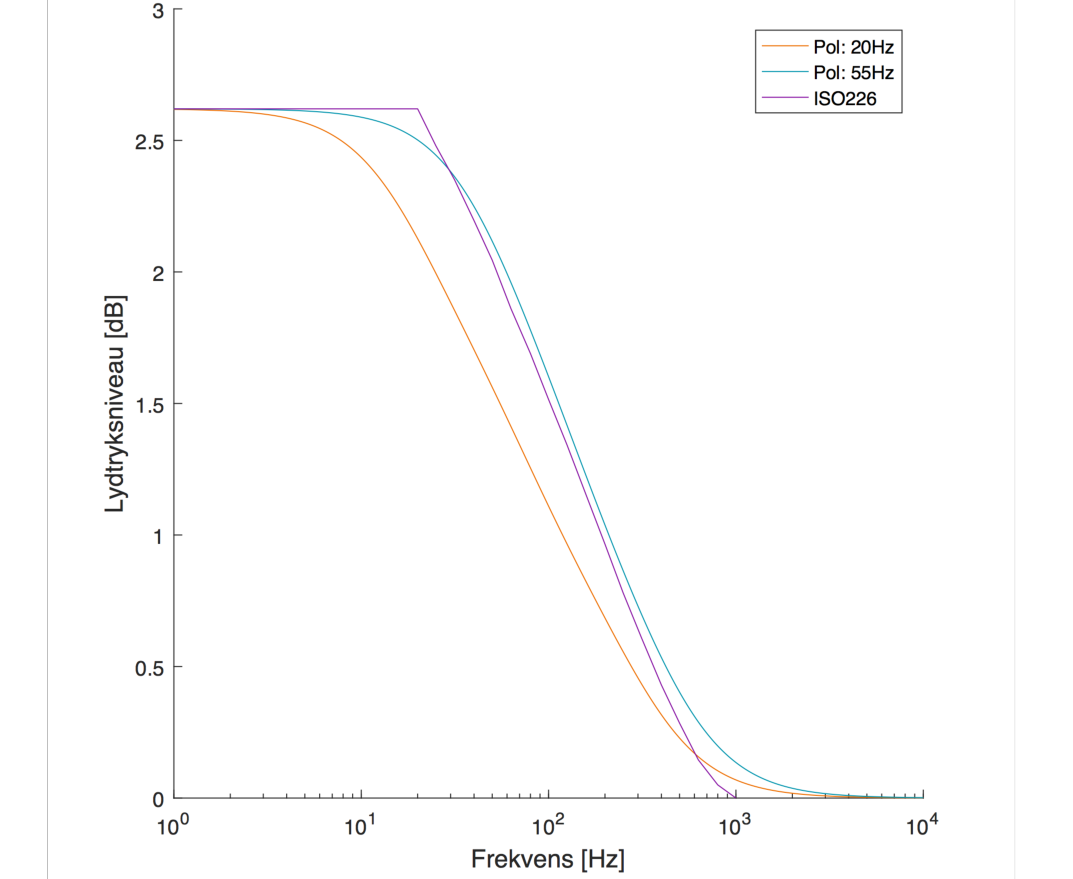
\includegraphics[resolution=300,width=\textwidth]{Figure/DesignAfFilter/JusteretPolSHORT.pdf}
	\caption{Justering af modstands- og kondensatorværdier for tre RC-led i forhold til ISO226.}
	\label{fig:JusteretPol}
\end{figure}
\noindent
%
Designet af det filter der skal forstærke 20Hz med 2.62dB, bliver udviklet i henhold til de foregående udregninger, som resulterer i kurven for 55Hz på \autoref{fig:JusteretPol}. Dertil bliver de restende filtre udviklet i henhold til de beregninger der foretages i de efterfølgende afsnits vedrørende dimensionering.
%
\begin{figure}[H]
	\centering
	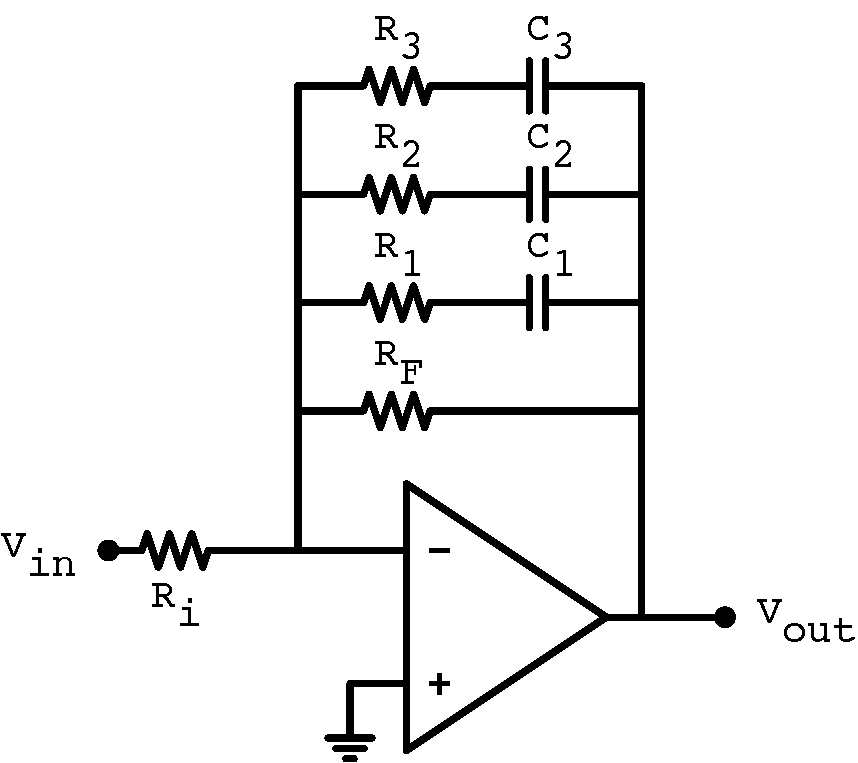
\includegraphics[resolution=300,scale=\circuitSize]{Figure/DesignAfFilter/FilterWith3.pdf}
	\caption{Kredsløbsdiagram for de fire filtre der skal forstærke de lave frekvenser.}
	\label{fig:ElDiagramFor3RC}
\end{figure}
\noindent
%
\newpage
\noindent
%
Uanset hvilken forstærkning modstandende og kondensatorværdierne bliver udregnet fra, så er kredsløbsdiagrammet på \autoref{fig:ElDiagramFor3RC} gældende for alle.
%

\subsection{Dimensionering af filter med 5.24dB's forstærkning}
\label{DimensioneringAfFilter5.24}
%
Fremgangsmåden for dimensionering af det filter der skal forstærke med 5.24dB er præcis den samme, som ved \fullref{DimensioneringAfFilter2.62}, dog tages der udgangspunkt i en anden forstærkning, de fuldkomne beregninger er vedlagt i \autoref{app:3RCledGain5.24}. For ikke at skulle gennemgå alle beregningerne igen, listes værdierne i de efterfølgende tabeller
%
\begin{table}[H]
\centering
\begin{tabular}{|r|r|r|r|r|r|r|r|}
\hline
\multicolumn{1}{|l|}{$G_{0dB}$} & \multicolumn{1}{l|}{$G_{1dB}$} & \multicolumn{1}{l|}{$G_{2dB}$} & \multicolumn{1}{l|}{$G_{3dB}$} & \multicolumn{1}{l|}{$G_0$} & \multicolumn{1}{l|}{$G_1$} & \multicolumn{1}{l|}{$G_2$} & \multicolumn{1}{l|}{$G_3$} \\ \hline
5.24dB & 3.493dB & 1.747dB & 0dB & 1.828 & 1.4951 & 1.2227 & 1\\ \hline
\end{tabular}
\caption{Oversigt over forstærkningen i dB og råforstærkningen, ved opdeling illustreret på \autoref{fig:GainOpdeling}.}
\label{tab:DimensioneringAf5.24Gain}
\end{table}
\noindent
%
%
\begin{table}[H]
\centering
\begin{tabular}{|r|r|r|r|r|r|r|}
\hline
\multicolumn{1}{|l|}{$R_F$} & \multicolumn{1}{l|}{$R_F'$} & \multicolumn{1}{l|}{$R_F''$} & \multicolumn{1}{l|}{$R_F'''$} & \multicolumn{1}{l|}{$R_1$} & \multicolumn{1}{l|}{$R_2$} & \multicolumn{1}{l|}{$R_3$} \\ \hline
18.281k$\Omega$ & 14.951k$\Omega$ & 12.227k$\Omega$ & 10k$\Omega$ & 82.074k$\Omega$ & 67.123k$\Omega$ & 54.896$k\Omega$\\ \hline
\end{tabular}
\caption{Oversigt over tilbagekoblingsmodstandene og de tre andre modstande.}
\label{tab:DimensioneringAf5.24Modstand}
\end{table}
\noindent
%

%
\begin{table}[H]
\centering
\begin{tabular}{|r|r|r|r|r|r|r|}
\hline
\multicolumn{1}{|l|}{$p_1$} & \multicolumn{1}{l|}{$p_2$} & \multicolumn{1}{l|}{$p_3$} & \multicolumn{1}{l|}{$p_4$} & \multicolumn{1}{l|}{$C_1$} & \multicolumn{1}{l|}{$C_2$} & \multicolumn{1}{l|}{$C_3$} \\ \hline
55Hz & 144.624Hz & 380.295Hz & 1000Hz & 28.835nF & 13.408nF & 6.235nF \\ \hline
\end{tabular}
\caption{Oversigt over knækfrevkserne for polerne og kondensatorværdierne.}
\label{tab:DimensioneringAf5.24polC}
\end{table}
\noindent
%

\subsection{Dimensionering af filter med 10.48dB's forstærkning}
\label{DimensioneringAfFilter10.48}
% 
Fremgangsmåden for dimensionering af det filter der skal forstærke med 10.48dB er præcis den samme, som ved \fullref{DimensioneringAfFilter2.62}, dog tages der udgangspunkt i en anden forstærkning, de fuldkomne beregninger er vedlagt i \autoref{app:3RCledGain10.48}. For ikke at skulle gennemgå alle beregningerne igen, listes værdierne i de efterfølgende tabeller
%
\begin{table}[H]
\centering
\begin{tabular}{|r|r|r|r|r|r|r|r|}
\hline
\multicolumn{1}{|l|}{$G_{0dB}$} & \multicolumn{1}{l|}{$G_{1dB}$} & \multicolumn{1}{l|}{$G_{2dB}$} & \multicolumn{1}{l|}{$G_{3dB}$} & \multicolumn{1}{l|}{$G_0$} & \multicolumn{1}{l|}{$G_1$} & \multicolumn{1}{l|}{$G_2$} & \multicolumn{1}{l|}{$G_3$} \\ \hline
10.48dB & 6.987dB & 3.493dB & 0dB & 3.342 & 2.2353 & 1.4951 & 1\\ \hline
\end{tabular}
\caption{Oversigt over forstærkningen i dB og råforstærkningen, ved opdeling illustreret på \autoref{fig:GainOpdeling}.}
\label{tab:DimensioneringAf10.48Gain}
\end{table}
\noindent
%
%
\begin{table}[H]
\centering
\begin{tabular}{|r|r|r|r|r|r|r|}
\hline
\multicolumn{1}{|l|}{$R_F$} & \multicolumn{1}{l|}{$R_F'$} & \multicolumn{1}{l|}{$R_F''$} & \multicolumn{1}{l|}{$R_F'''$} & \multicolumn{1}{l|}{$R_1$} & \multicolumn{1}{l|}{$R_2$} & \multicolumn{1}{l|}{$R_3$} \\ \hline
33.42k$\Omega$ & 22.353k$\Omega$ & 14.951k$\Omega$ & 10k$\Omega$ & 67.502k$\Omega$ & 45.149k$\Omega$ & 30.198k$\Omega$\\ \hline
\end{tabular}
\caption{Oversigt over tilbagekoblingsmodstandene og de tre andre modstande.}
\label{tab:DimensioneringAf10.48Modstand}
\end{table}
\noindent
%
%
\begin{table}[H]
\centering
\begin{tabular}{|r|r|r|r|r|r|r|}
\hline
\multicolumn{1}{|l|}{$p_1$} & \multicolumn{1}{l|}{$p_2$} & \multicolumn{1}{l|}{$p_3$} & \multicolumn{1}{l|}{$p_4$} & \multicolumn{1}{l|}{$C_1$} & \multicolumn{1}{l|}{$C_2$} & \multicolumn{1}{l|}{$C_3$} \\ \hline
55Hz & 144.624Hz & 380.295Hz & 1000Hz & 28.673nF & 16.303nF & 9.269nF \\ \hline
\end{tabular}
\caption{Oversigt over knækfrevkserne for polerne og kondensatorværdierne.}
\label{tab:DimensioneringAf10.48polC}
\end{table}
\noindent
%
%
\subsection{Dimensionering af filter med 20.96dB's forstærkning}
\label{DimensioneringAfFilter20.96}
%
Fremgangsmåden for dimensionering af det filter der skal forstærke med 20.96dB er præcis den samme, som ved \fullref{DimensioneringAfFilter2.62}, dog tages der udgangspunkt i en anden forstærkning, de fuldkomne beregninger er vedlagt i \autoref{app:3RCledGain20.96}. For ikke at skulle gennemgå alle beregningerne igen, listes værdierne i de efterfølgende tabeller
%
\begin{table}[H]
\centering
\begin{tabular}{|r|r|r|r|r|r|r|r|}
\hline
\multicolumn{1}{|l|}{$G_{0dB}$} & \multicolumn{1}{l|}{$G_{1dB}$} & \multicolumn{1}{l|}{$G_{2dB}$} & \multicolumn{1}{l|}{$G_{3dB}$} & \multicolumn{1}{l|}{$G_0$} & \multicolumn{1}{l|}{$G_1$} & \multicolumn{1}{l|}{$G_2$} & \multicolumn{1}{l|}{$G_3$} \\ \hline
20.96dB & 13.973dB & 6.987dB & 0dB & 11.169 & 4.9965 & 2.2353 & 1\\ \hline
\end{tabular}
\caption{Oversigt over forstærkningen i dB og råforstærkningen, ved opdeling illustreret på \autoref{fig:GainOpdeling}.}
\label{tab:DimensioneringAf20.96Gain}
\end{table}
\noindent
%
%
\begin{table}[H]
\centering
\begin{tabular}{|r|r|r|r|r|r|r|}
\hline
\multicolumn{1}{|l|}{$R_F$} & \multicolumn{1}{l|}{$R_F'$} & \multicolumn{1}{l|}{$R_F''$} & \multicolumn{1}{l|}{$R_F'''$} & \multicolumn{1}{l|}{$R_1$} & \multicolumn{1}{l|}{$R_2$} & \multicolumn{1}{l|}{$R_3$} \\ \hline
111.686k$\Omega$ & 49.965k$\Omega$ & 22.353k$\Omega$ & 10k$\Omega$ & 90.413k$\Omega$ & 40.448k$\Omega$ & 18.095k$\Omega$\\ \hline
\end{tabular}
\caption{Oversigt over tilbagekoblingsmodstandene og de tre andre modstande.}
\label{tab:DimensioneringAf20.96Modstand}
\end{table}
\noindent
%
%
\begin{table}[H]
\centering
\begin{tabular}{|r|r|r|r|r|r|r|}
\hline
\multicolumn{1}{|l|}{$p_1$} & \multicolumn{1}{l|}{$p_2$} & \multicolumn{1}{l|}{$p_3$} & \multicolumn{1}{l|}{$p_4$} & \multicolumn{1}{l|}{$C_1$} & \multicolumn{1}{l|}{$C_2$} & \multicolumn{1}{l|}{$C_3$} \\ \hline
55Hz & 144.624Hz & 380.295Hz & 1000Hz & 14.318nF & 12.172nF & 10.347nF \\ \hline
\end{tabular}
\caption{Oversigt over knækfrevkserne for polerne og kondensatorværdierne.}
\label{tab:DimensioneringAf20.96polC}
\end{table}
\noindent
%